\section{Sparse Regression Comparison and Outbreak-Curve Validation}
\label{sec:track-e}

This section compares two fundamentally different ways of discovering
governing equations from data -- sparse symbolic regression and gradient-based
neural fitting -- and separately tests whether the cross-domain stability
fixes of Section~\ref{sec:phase2} generalize beyond the mechanistic system
that produced them.

\subsection{Noise robustness: KAN-ODE vs.\ sparse symbolic regression}

Sparse Identification of Nonlinear Dynamics (SINDy) \cite{brunton2016sindy}
fits a governing equation as a sparse linear combination of candidate terms
drawn from a fixed library -- here, every polynomial in $x$ and $y$ up to
degree 2, i.e.\ $\{1,x,y,x^2,xy,y^2\}$. Coefficients are estimated by
sequentially thresholded least squares: an ordinary least-squares fit is
performed against numerically estimated derivatives, every coefficient
below a fixed threshold is zeroed out, and the fit is repeated on the
surviving terms until the active set stops changing. This is what makes the
recovered model sparse and, in principle, human-readable -- unlike the KAN's
240 free parameters, SINDy returns a short list of surviving terms with
numeric coefficients attached, directly comparable to the true equation's
own coefficients. The coefficient threshold is held fixed across the entire
noise sweep so that the comparison measures noise sensitivity rather than
per-level tuning. It is fit against the same noise-corrupted Lotka-Volterra
observations the earlier KAN checkpoints (Section~\ref{sec:phase2}) were
trained on, scored against clean ground truth.

\begin{expectbox}
\expectrow{Question}{How does a sparse, symbolic method compare to a dense, 240-parameter neural method as observation noise increases?}
\expectrow{Expected}{Sparse regression's tiny library should make it more robust to noise; KAN-ODE's larger parameter count should make it more accurate.}
\expectrow{Observed}{Both expectations hold, but the KAN-ODE advantage collapses $170\times$ across the sweep, from $1110\times$ at zero noise to $6.5\times$ at $\sigma=0.1$.}
\end{expectbox}

\begin{table}[!ht]
\centering
\small
\renewcommand{\arraystretch}{1.1}
\caption{Extrapolation MSE vs.\ observation noise $\sigma$.}
\label{tab:sindy-noise}
\begin{tabularx}{\textwidth}{@{}C{1.3cm} C{2.6cm} C{2.6cm} X@{}}
\toprule
\hdrrow \thh{Noise level $\sigma$} & \thh{Sparse regression} & \thh{KAN-ODE} & \thh{KAN-ODE advantage}\\
\midrule
0.00 & $9.90\times10^{-2}$ & $\mathbf{8.92\times10^{-5}}$ & $1110\times$\\
0.01 & $1.58\times10^{-1}$ & $1.22\times10^{-3}$ & $130\times$\\
0.05 & $1.48\times10^{-1}$ & $2.54\times10^{-2}$ & $5.8\times$\\
0.10 & $8.89\times10^{-1}$ & $1.37\times10^{-1}$ & $6.5\times$\\
\bottomrule
\end{tabularx}
\end{table}

\begin{figure}[htbp]
\centering
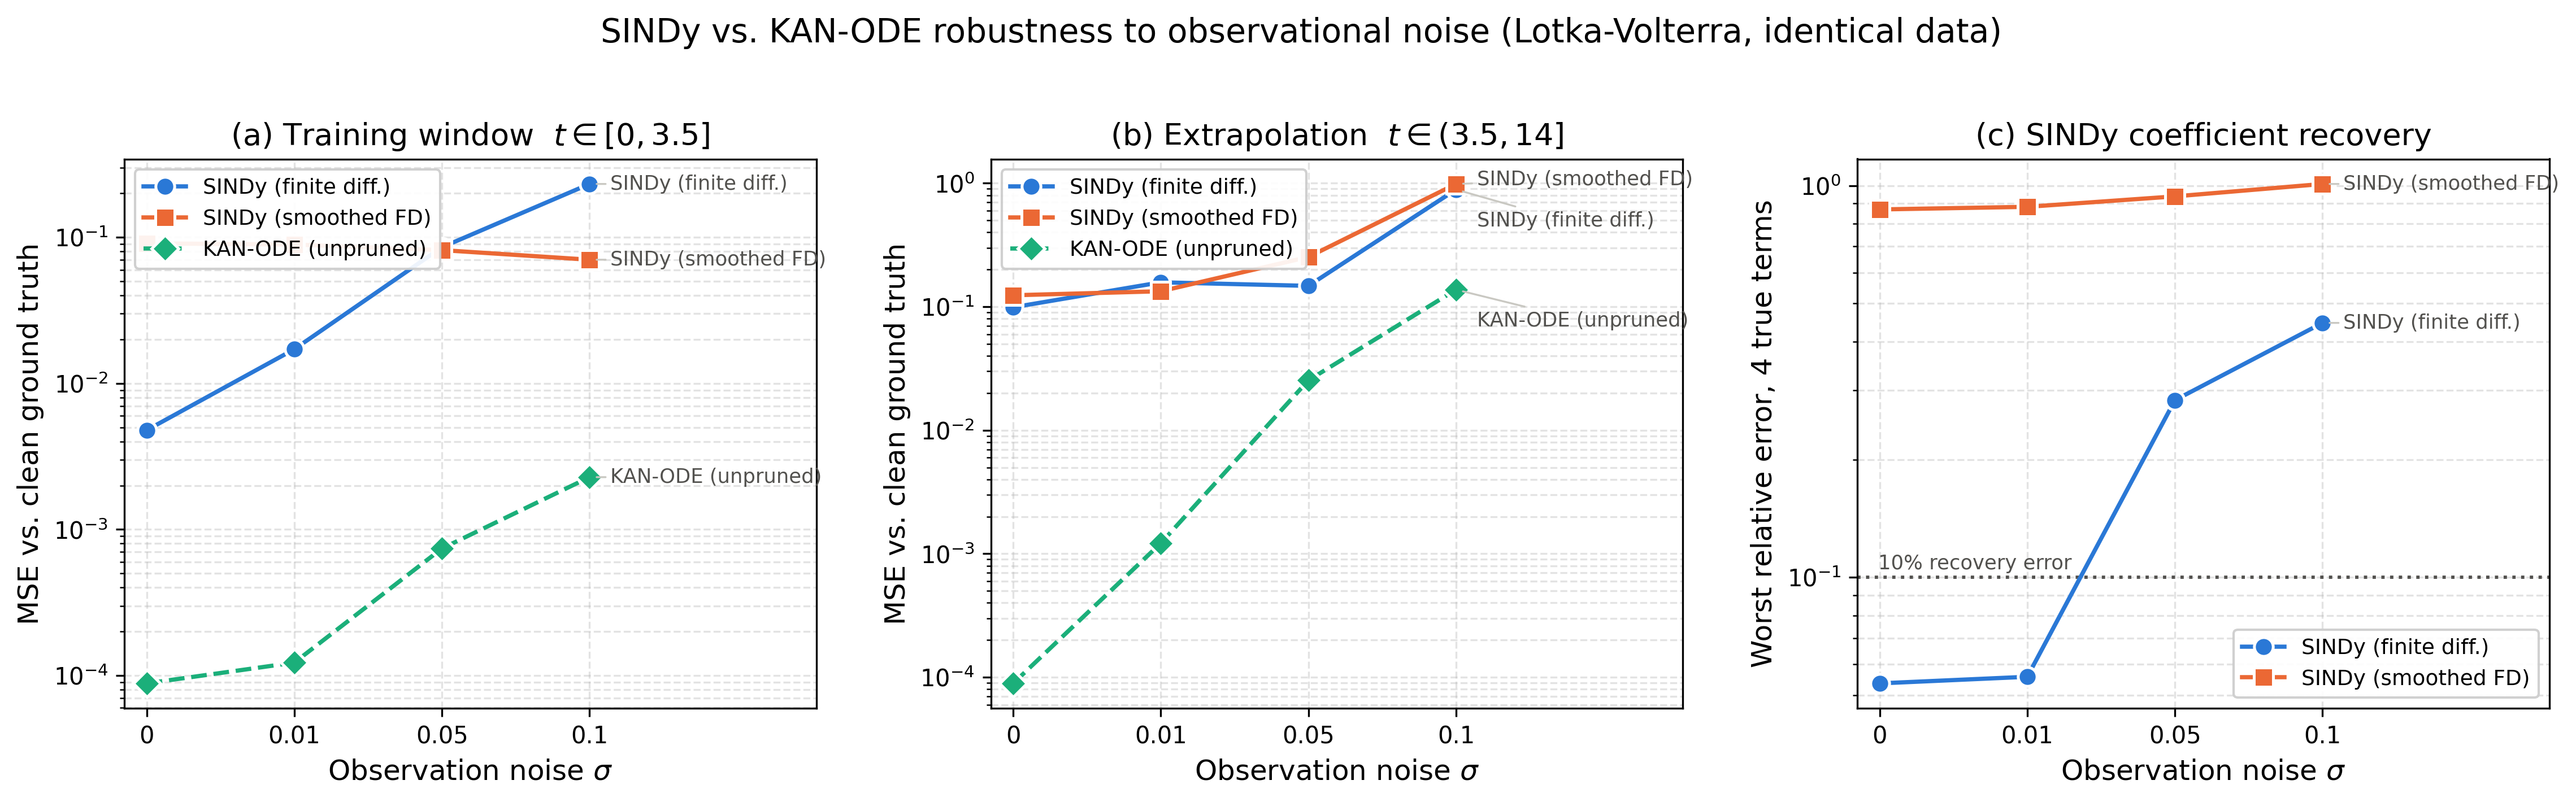
\includegraphics[width=0.8\linewidth]{figures/track_e/sindy_vs_kan_noise.png}
\caption{Training and extrapolation MSE vs.\ noise level, both methods.}
\label{fig:sindy-noise}
\end{figure}

KAN-ODE wins on absolute accuracy at every level, but the margin collapses
$170\times$ across the sweep (sparse regression degrades $9.0\times$ from
$\sigma=0$ to $0.1$; KAN-ODE degrades $1540\times$). The sparse regression's
six-term library caps how much noise can move it; the KAN's 240 free
parameters fit the noise directly and the error compounds through the
solver. Per-term recovery shows the bilinear cross-term ($xy$) is recovered
to within $5.7\%$ at every noise level -- exactly the term a single-layer KAN
edge, being strictly univariate, cannot represent directly, since each edge
is a function of only one input variable and a layer sums its edges
additively. This asymmetry -- sparse regression writes $xy$ as a literal
library column, while a KAN can only approximate it through composition
across a hidden layer -- means a term-by-term symbolic comparison would be
comparing a coefficient against a distributed representation, so the
comparison used here is trajectory reconstruction instead.

\begin{figure}[htbp]
\centering
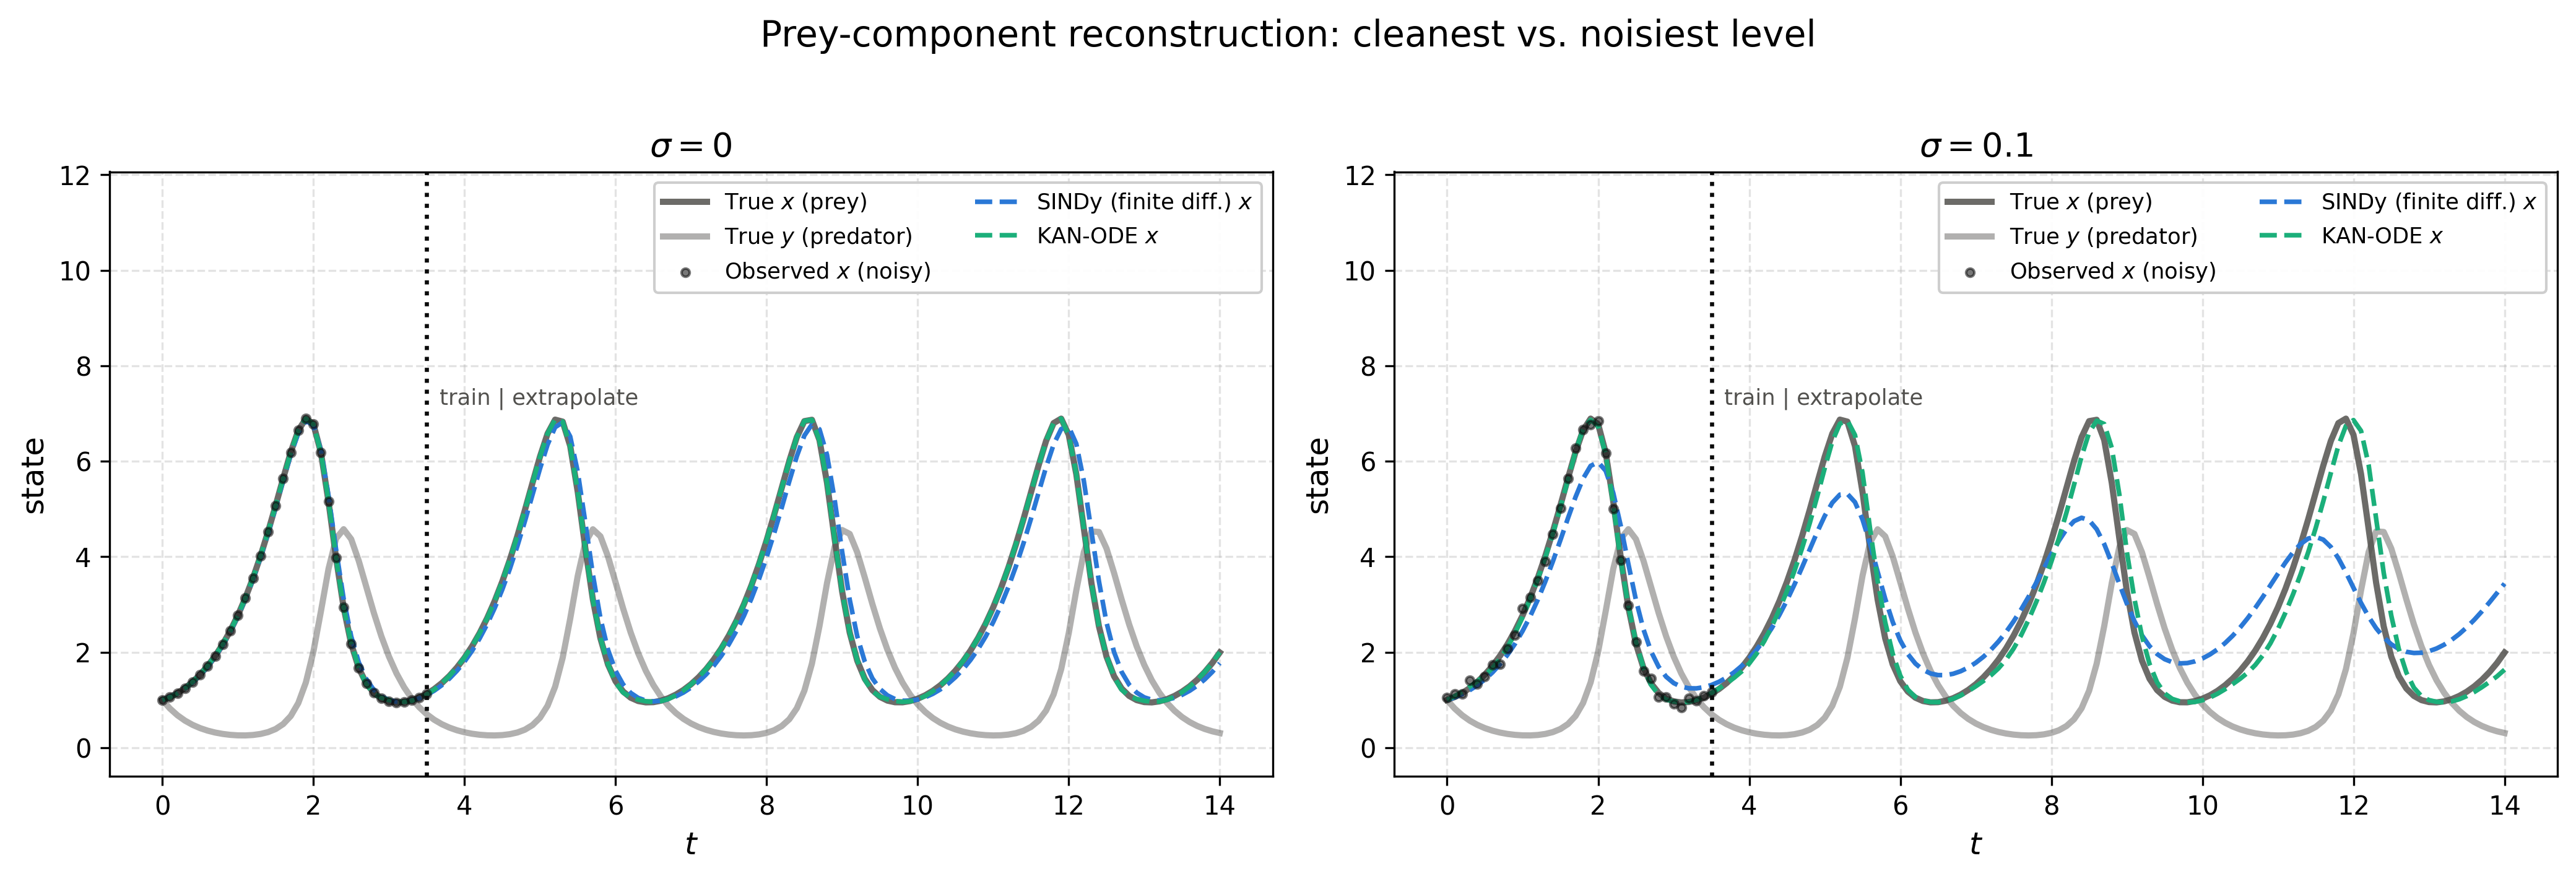
\includegraphics[width=0.8\linewidth]{figures/track_e/sindy_vs_kan_trajectories.png}
\caption{Reconstructed trajectories at $\sigma=0$ and $\sigma=0.1$: sparse
regression loses amplitude under noise; KAN-ODE keeps amplitude but drifts
in phase.}
\label{fig:sindy-trajectories}
\end{figure}

\subsection{Edge pruning: testing whether a term-by-term comparison is even possible}

Part of the original motivation for a smooth, globally-supported basis such
as RBF is that a sparse, pruned KAN edge structure could in principle be read
back as a closed-form symbolic law, the same interpretability goal sparse
regression achieves by construction. The base paper reaches this by adding an
$L_1$ penalty on every spline coefficient to the training loss,
\begin{equation}
\mathcal{L} = \mathrm{MSE}(\mathbf{u}_{\text{true}}, \mathbf{u}_{\text{pred}}) + \lambda\sum_{i} |c_i|,
\label{eq:l1-sparsity}
\end{equation}
where $c_i$ ranges over every spline coefficient in Equation~\ref{eq:kan-edge}
and $\lambda$ trades off trajectory accuracy against how many edges the
penalty drives toward zero. Every checkpoint trained for this project used
$\lambda=0$: the plain mean-squared-error term alone, with no sparsity
pressure ever added to Equation~\ref{eq:l1-sparsity}. A KAN-ODE analogue of a
sparse coefficient list would instead come from pruning weak edges
\emph{post hoc} and reading off what survives. Ranking each edge by mean
spline-coefficient magnitude and masking the weakest, applied to the existing
(never retrained) noise-sweep checkpoints, removes the two weakest of forty
edges and raises the noise-free full-horizon MSE from $8.90\times10^{-5}$ to
$3.43$ -- a factor of $3.9\times10^{4}$, worse than predicting the constant
dataset mean ($2.91$). Every checkpoint was trained with no sparsity-inducing
regularization applied at all, so nothing during training ever asked the
network to concentrate its fit onto a few edges; the flat plateau at
$\approx3.5$--$3.8$ across all pruning levels of 25\% or more is the
signature of a model where every edge carries part of the fit, confirming
that the pruning procedure itself works correctly on a network that has no
prunable structure to find.

\begin{figure}[htbp]
\centering
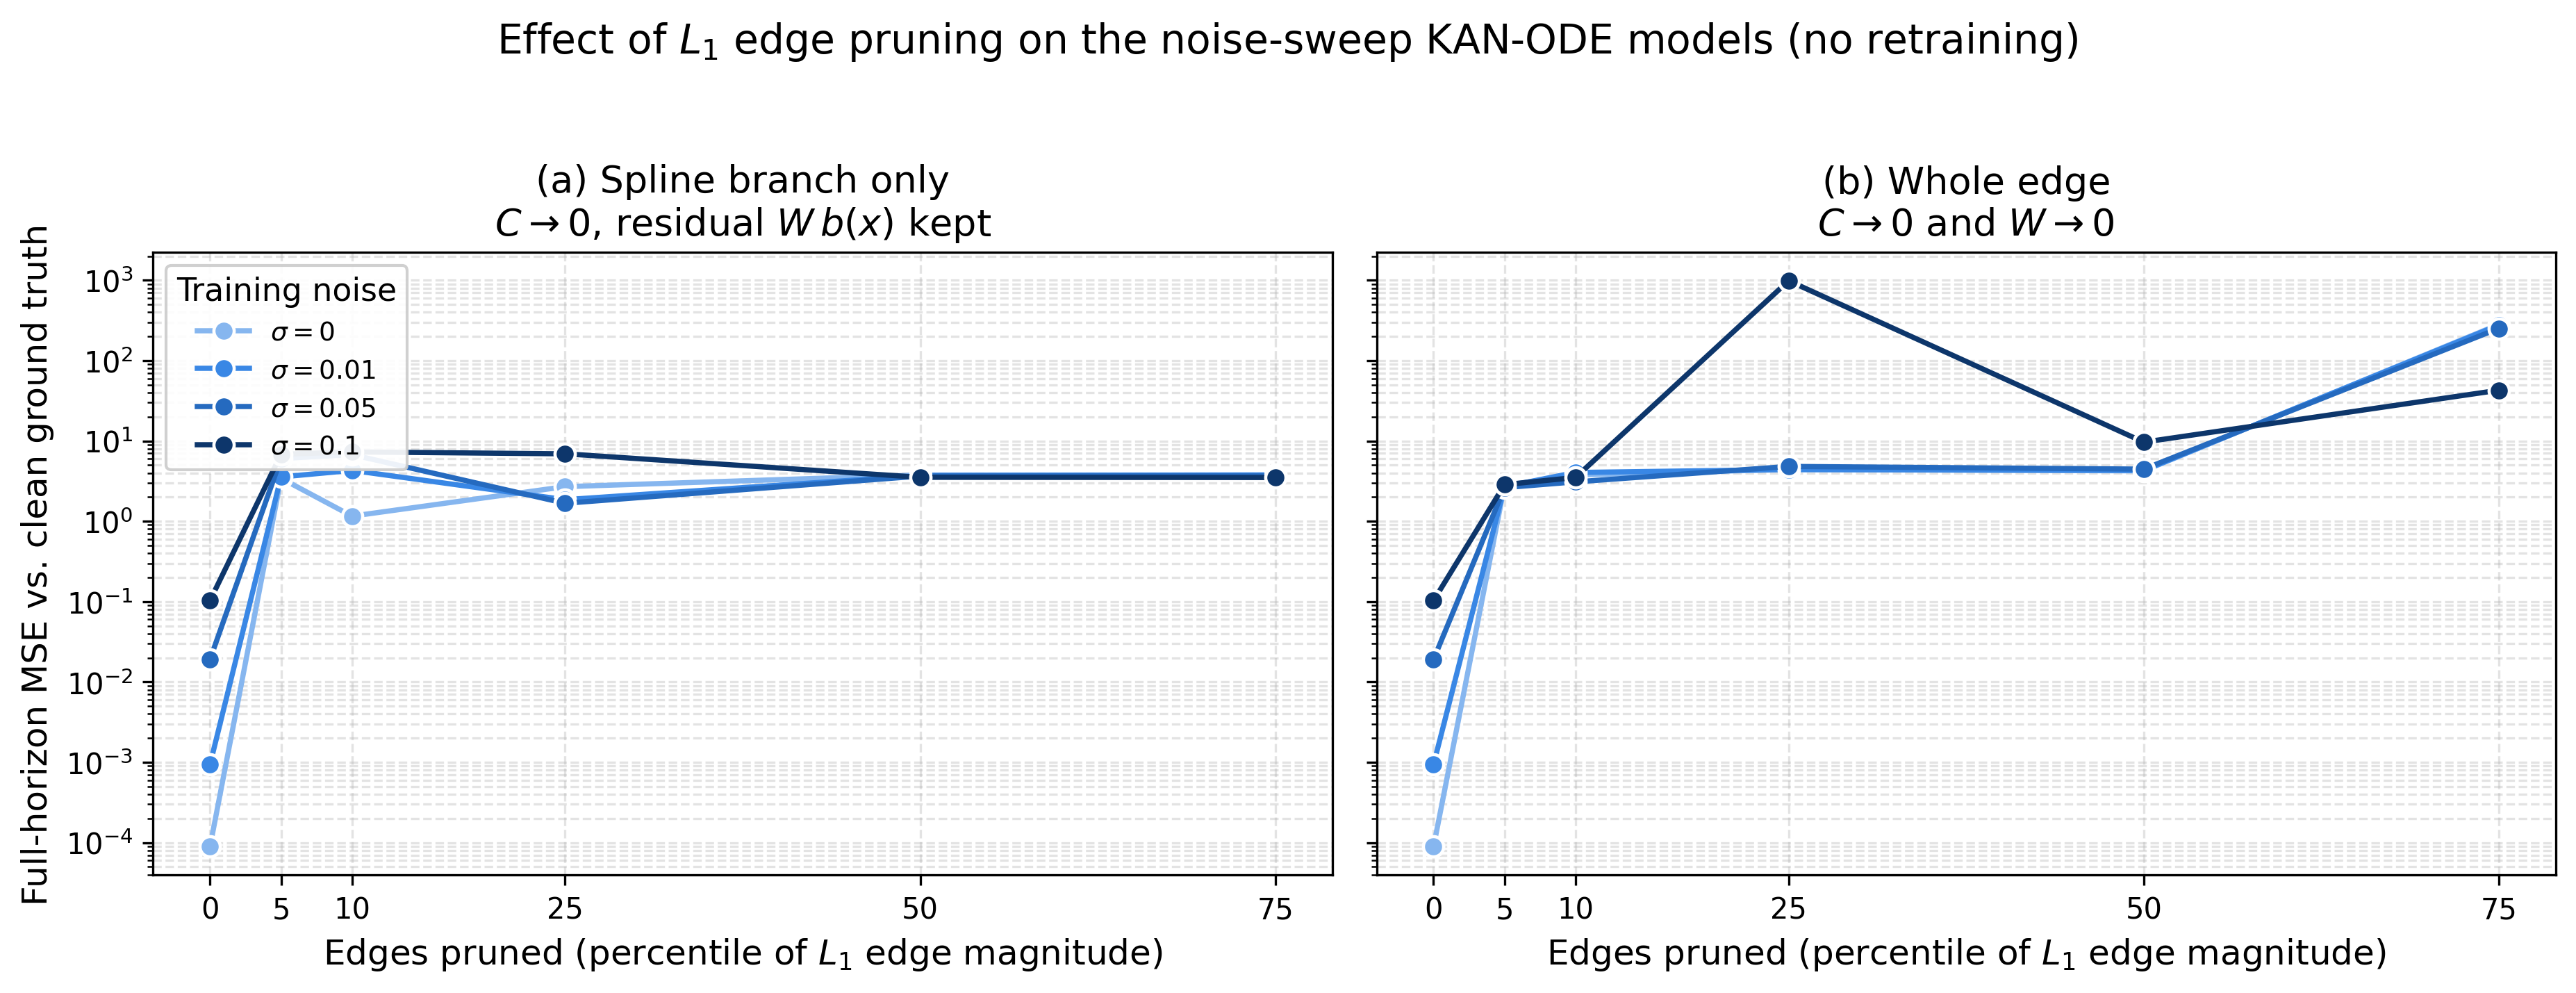
\includegraphics[width=0.8\linewidth]{figures/track_e/pruning_degradation.png}
\caption{Full-horizon MSE vs.\ edge-pruning fraction, all four noise levels.}
\label{fig:pruning}
\end{figure}

\subsection{Testing whether SIR's fixes transfer to a non-mechanistic epidemic curve}

A single outbreak wave that no compartmental ODE generated tests whether the SIR fixes of
Section~\ref{sec:phase2} generalize by mechanism rather than by coincidence
of the SIR system's own structure. The curve is synthetic but shaped like
observed case data: a Gaussian wave centred at day 38 and skewed so that
its infected peak falls on day 45, with $1\%$
observation noise and a 7-day moving average, spanning 120 days, of which
the first 45 are used for training. The same init-time diagnostic used to
root-cause SIR reproduces an almost identical speed-mismatch signature
($18.77\times$ vs.\ SIR's $19\times$), justifying a time rescaling by a
factor of 24 \emph{a priori}, before any training.

\begin{expectbox}
\expectrow{Question}{SIR's three stability fixes were each derived from a property of the SIR generator itself -- do they still work on data no compartmental model produced?}
\expectrow{Expected}{Only the unit-rescaling fix, which assumes nothing about the data's structure, should transfer; the two structural fixes should not.}
\expectrow{Observed}{One in three predictions was wrong: the vanishing-field gate transfers and is the best single option, despite being predicted inapplicable.}
\end{expectbox}

\begin{table}[!ht]
\centering
\small
\renewcommand{\arraystretch}{1.15}
\caption{Which of SIR's three fixes transfer to a non-mechanistic curve.}
\label{tab:fix-transfer}
\begin{tabularx}{\textwidth}{@{}L{3.4cm} L{4.4cm} C{1.6cm} X@{}}
\toprule
\hdrrow \thh{Fix} & \thh{Precondition} & \thh{Holds?} & \thh{Outcome}\\
\midrule
Time rescaling & None -- a unit change & Yes & Removes a $263{,}049\times$ gradient spike\\
Conservation via subspace projection & An exact invariant, $\sum y=c$ & No ($\sum y$ spans $0.002$--$1.54$) & Inapplicable; $25\times$ worse fit\\
Vanishing-field gate at the equilibrium point & $y_d=0$ is a manifold of equilibria & Yes (unexpectedly) & Best single option, $47\times$ better fit\\
\bottomrule
\end{tabularx}
\end{table}

The vanishing-field gate was \emph{predicted} inapplicable: the infected
fraction at $t=0$ is $0.0027$, seemingly too small to avoid freezing the
field entirely. A control arm overturns that prediction: gating the learned
field by the initial state correctly encodes that the rate of change is
proportional to current prevalence, and is the only configuration that
reproduces the existence of a peak (day 48 predicted vs.\ true day 45) from a
training window that never observed one.

\begin{figure}[htbp]
\centering
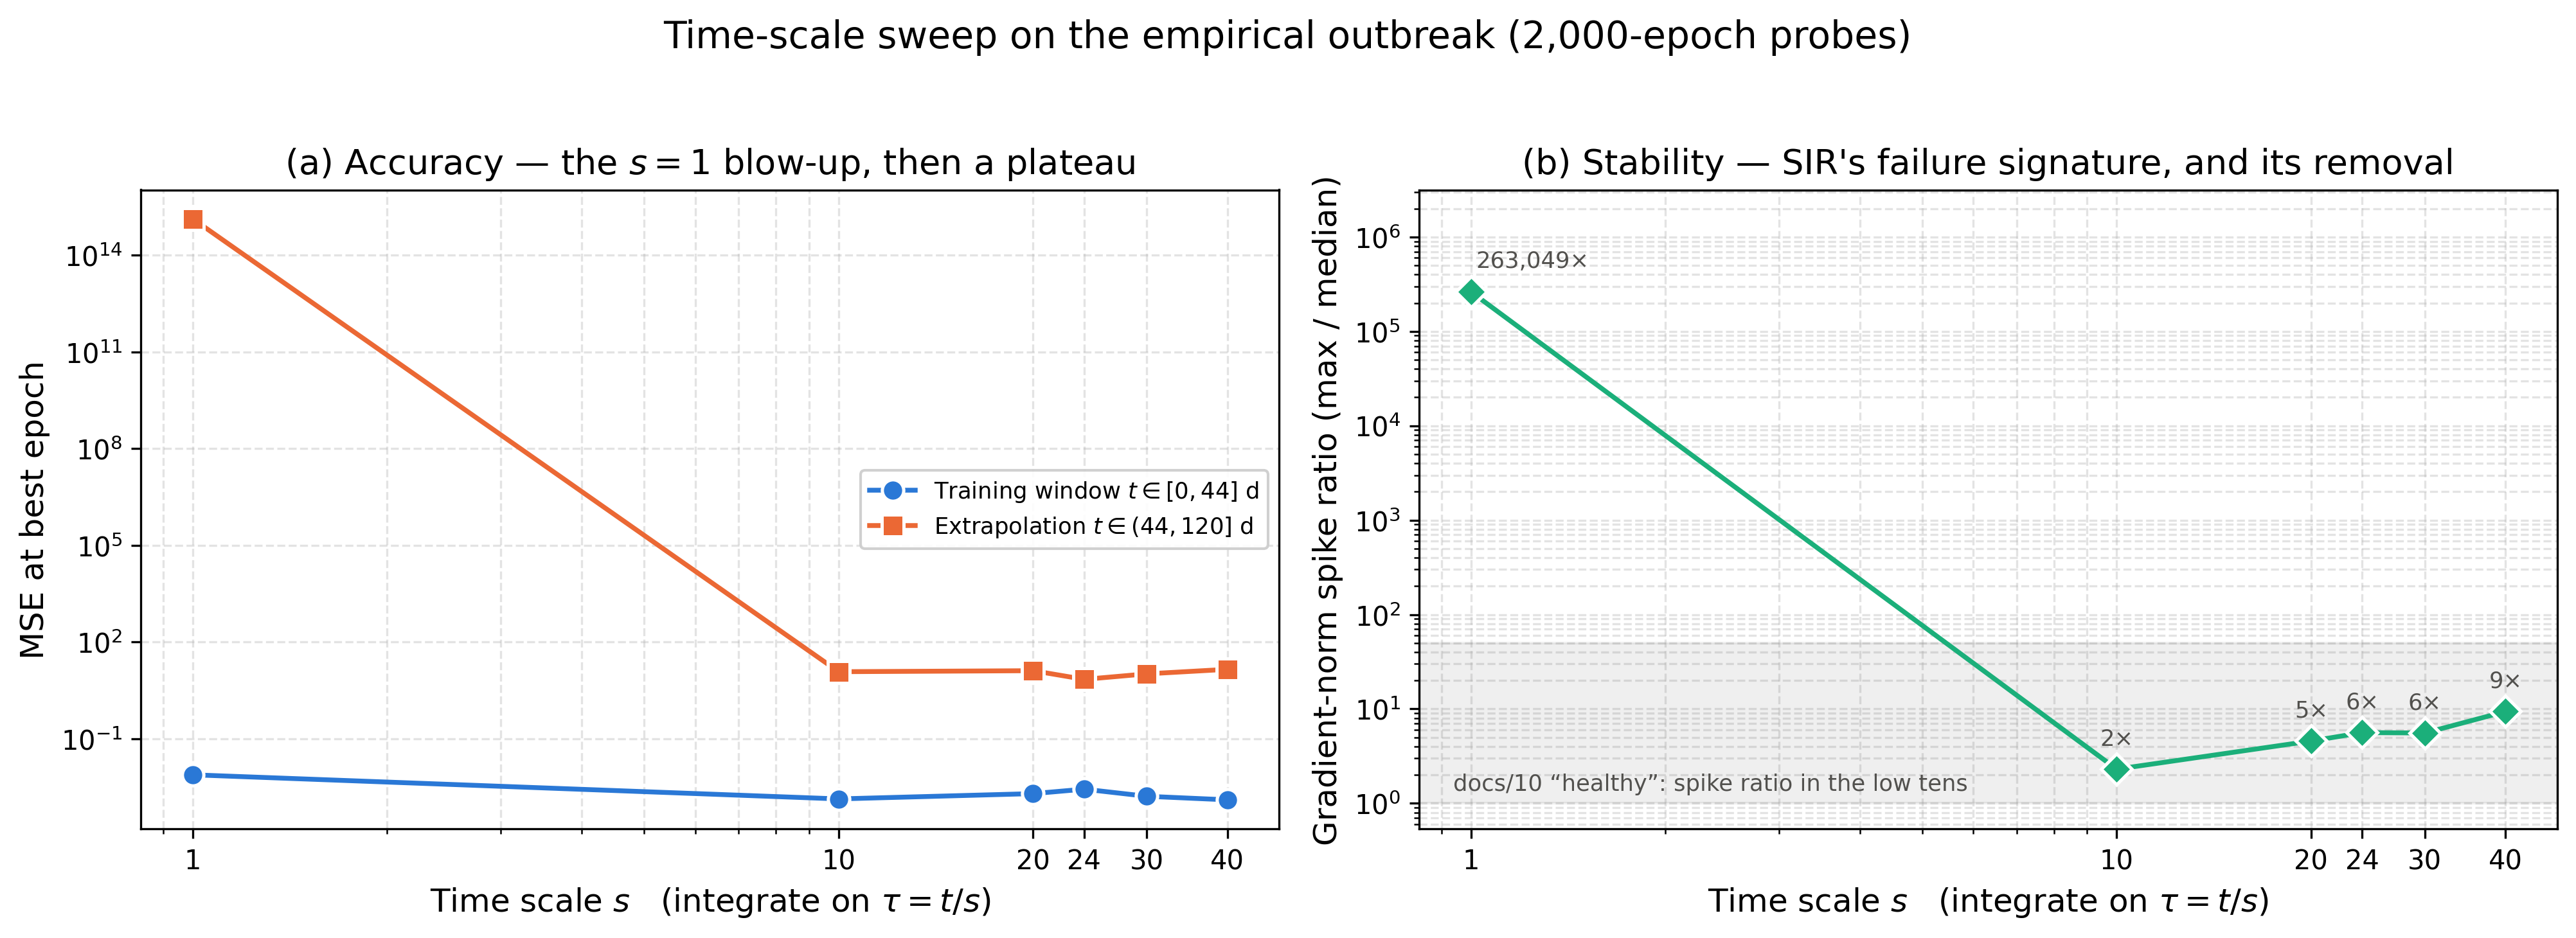
\includegraphics[width=0.8\linewidth]{figures/track_e/epidemic_time_scale_sweep.png}
\caption{Time-rescaling sweep: accuracy and gradient-spike ratio vs.\ the
rescaling factor.}
\label{fig:time-scale-sweep}
\end{figure}

\paragraph{The extrapolation runaway traces to the train/test split.} The
default split lands exactly on the infected peak (0\% of the decay phase is
in the training window), so every model is asked to predict a monotone decay
it has never observed. Moving the split just 15 days later collapses the
predicted maximum from $6.18\times$ the true peak to $0.964$ (true maximum
$=1.0$), turning over at day 47 against a true day 45 -- the runaway is a
property of where the window ends, not of the method fitting the data.

\begin{figure}[htbp]
\centering
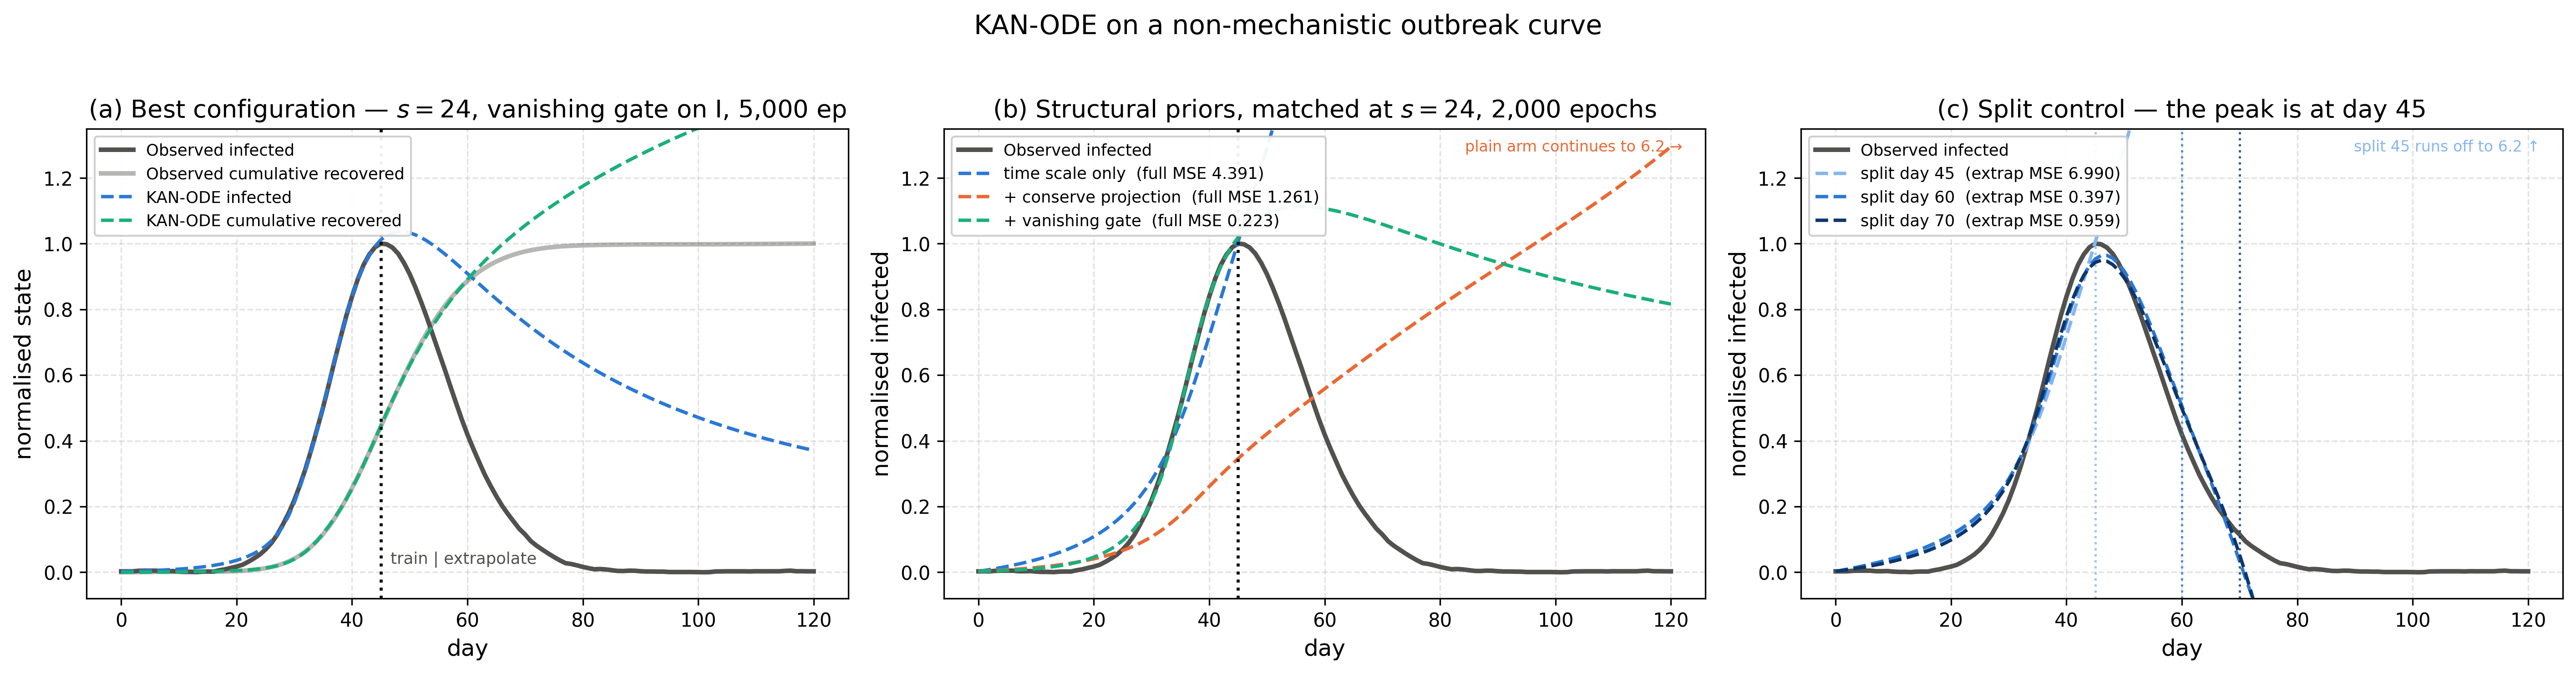
\includegraphics[width=0.8\linewidth]{figures/track_e/real_epidemic_fit.png}
\caption{Outbreak-curve fit: default split (runaway), the vanishing-field-gate
arm, and the fifteen-day-later split control.}
\label{fig:real-epidemic-fit}
\end{figure}

\begin{keypoint}[Verdict]
Time rescaling transfers unconditionally because it is a unit change with no
structural precondition. The other two fixes are structural priors that
transfer exactly insofar as their structure is actually present in the new
data: the conservation projection's precondition is confirmable in advance
by directly measuring the compartment sum, while the vanishing-field gate's
precondition turned out to require running the control arm to settle --
argument alone predicted the wrong outcome. That arm cost 27 minutes and
overturned the prediction.
\end{keypoint}

\FloatBarrier
